\subsection{Distributed SGF FW Experiments}
To test the performance of Algorithm \ref{distributed} we used 10 workers and an adjacecy matrix $A$ given by
\[ A =
\begin{pmatrix}
1& 1& 0& 1& 1& 1& 1& 1& 0& 1\\
1& 1& 1& 0& 1& 1& 1& 0& 1& 1\\
0& 1& 1& 1& 1& 1& 0& 1& 1& 1\\
1& 0& 1& 1& 1& 1& 0& 1& 1& 1\\
1& 1& 1& 1& 1& 1& 1& 0& 1& 1\\
1& 1& 1& 1& 1& 1& 1& 1& 1& 0\\
1& 1& 0& 0& 1& 1& 1& 1& 1& 1\\
1& 0& 1& 1& 0& 1& 1& 1& 1& 1\\
0& 1& 1& 1& 1& 1& 1& 1& 1& 1\\
1& 1& 1& 1& 1& 0& 1& 1& 1& 1
\end{pmatrix}
.\]
We can notice that the diagonal is of ones, this because each node is connected to itself. Our network is composed of
10 nodes and the connectivity of the graph can be know by computing $\Vert W- J \Vert$, where $J= 11^T/10$ and $11^T$
represent a matrix with all entries set to 1. In our case we have a connectivity value of 0.438. We use 15 directions
and test the algorithm for 20, 50 and 100 queries.

\begin{figure}[htbp]
	\centering
	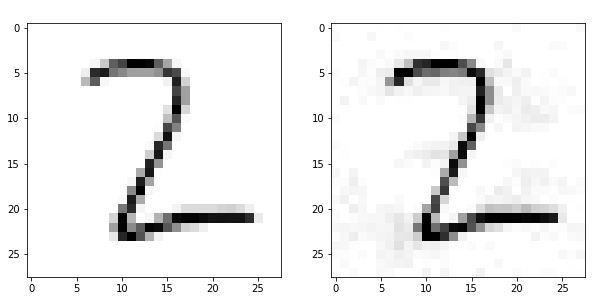
\includegraphics[width=7cm]{image_pertub_T100_final_distr.png}
	\caption{Image of 2 changed to 3 with the adversarial perturbation generated by the Distributed Algorithm \ref{distributed} with 100 queries.}
	\label{fig:distributed}
\end{figure}

\begin{figure}%[htbp]
	\centering
	\begin{subfigure}[b]{0.15\textwidth}
		\centering
		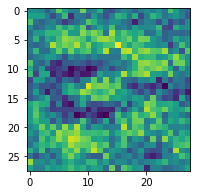
\includegraphics[width=2.5cm]{T20_final_distr.png}
		\caption{}
		\label{fig:decentralized_perturbation}
	\end{subfigure}
	\hfill
	\begin{subfigure}[b]{0.15\textwidth}
		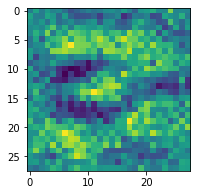
\includegraphics[width=2.5cm]{T50_final_distr.png}
		\caption{}
		\label{fig:variance-reduce_perturbation}
	\end{subfigure}
	\hfill
	\begin{subfigure}[b]{0.15\textwidth}
		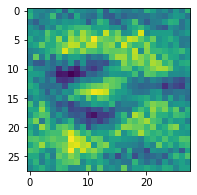
\includegraphics[width=2.5cm]{T100_final_distr.png}
		\caption{}
		\label{fig:distributed_perturbation}
	\end{subfigure}
	\caption{Perturbations of the Distributed SGF FW algorithm: \ref{fig:decentralized_perturbation} is the perturbation with T=20, \ref{fig:variance-reduce_perturbation} is the perturbation with T=50, \ref{fig:distributed_perturbation} is the perturbation with T=100.}
	\label{fig:perturbations}
\end{figure}